\documentclass{standalone}
\usepackage{tikz}
\usetikzlibrary{shapes.geometric}
\begin{document}
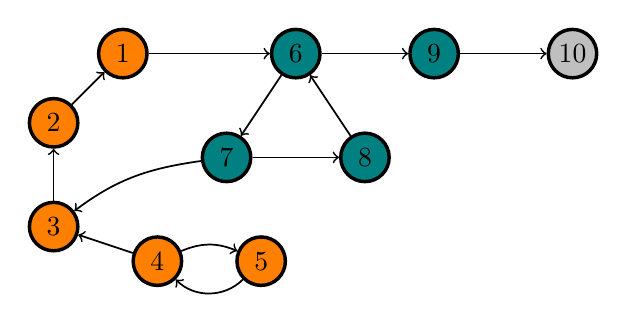
\begin{tikzpicture}
[every node/.style={inner sep=0pt}]
\node (1) [circle, minimum size=17.5pt, fill=orange, line width=1.25pt, draw=black] at (50.0pt, -12.5pt) {\textcolor{black}{1}};
\node (2) [circle, minimum size=17.5pt, fill=orange, line width=1.25pt, draw=black] at (25.0pt, -37.5pt) {\textcolor{black}{2}};
\node (3) [circle, minimum size=17.5pt, fill=orange, line width=1.25pt, draw=black] at (25.0pt, -75.0pt) {\textcolor{black}{3}};
\node (10) [circle, minimum size=17.5pt, fill=lightgray, line width=1.25pt, draw=black] at (212.5pt, -12.5pt) {\textcolor{black}{10}};
\node (9) [circle, minimum size=17.5pt, fill=teal, line width=1.25pt, draw=black] at (162.5pt, -12.5pt) {\textcolor{black}{9}};
\node (6) [circle, minimum size=17.5pt, fill=teal, line width=1.25pt, draw=black] at (112.5pt, -12.5pt) {\textcolor{black}{6}};
\node (7) [circle, minimum size=17.5pt, fill=teal, line width=1.25pt, draw=black] at (87.5pt, -50.0pt) {\textcolor{black}{7}};
\node (8) [circle, minimum size=17.5pt, fill=teal, line width=1.25pt, draw=black] at (137.5pt, -50.0pt) {\textcolor{black}{8}};
\node (4) [circle, minimum size=17.5pt, fill=orange, line width=1.25pt, draw=black] at (62.5pt, -87.5pt) {\textcolor{black}{4}};
\node (5) [circle, minimum size=17.5pt, fill=orange, line width=1.25pt, draw=black] at (100.0pt, -87.5pt) {\textcolor{black}{5}};
\draw [line width=0.625, ->, color=black] (2) to  (1);
\draw [line width=0.625, ->, color=black] (3) to  (2);
\draw [line width=0.625, ->, color=black] (4) to  (3);
\draw [line width=0.625, ->, color=black] (4) to  [in=157, out=23] (5);
\draw [line width=0.625, ->, color=black] (5) to  [in=315, out=225] (4);
\draw [line width=0.625, ->, color=black] (6) to  (7);
\draw [line width=0.625, ->, color=black] (7) to  (8);
\draw [line width=0.625, ->, color=black] (8) to  (6);
\draw [line width=0.625, ->, color=black] (6) to  (9);
\draw [line width=0.625, ->, color=black] (9) to  (10);
\draw [line width=0.625, ->, color=black] (1) to  (6);
\draw [line width=0.625, ->, color=black] (7) to  [in=37, out=188] (3);


\end{tikzpicture}

\end{document}
